\section{实验六}
    \subsection{题目}
        \begin{enumerate}
            \item 程序从下单页跳转到支付页调用了小程序提供的哪个 $api$ 函数?
                \begin{mquote}
                    \par 分别在 \textbf{pages/goods/detail/index.js} 和 \textbf{pages/cart/index.js} 中调用了微信小程序提供的 \textbf{\textit{wx.navigateTo}} 函数
                \end{mquote}
                \lstinputlisting[style = C++, title = {\bf pages/goods/detail/index.js}]{navi1.cpp}
                \lstinputlisting[style = C++, title = {\bf pages/goods/detail/index.js}]{navi2.cpp}
            \item 在小程序中完成页面跳转的都有哪些函数,都分别用于什么场合?
                \begin{mquote}
                    \begin{enumerate}
                        \item \textbf{wx.navigateTo} 函数
                            \begin{itemize}
                                \item 作用:保留当前的页面,并转跳到小程序内的其他页面中
                                \item 场合:在跳转页面的同时也需要保留原来页面的数据时可以使用
                            \end{itemize}
                        \item \textbf{wx.redirectTo} 函数
                            \begin{itemize}
                                \item 作用:关闭当前的页面,并转跳到小程序内的其他页面中
                                \item 场合:在跳转页面的同时不需要保留原来页面的数据时可以使用
                            \end{itemize}
                        \item \textbf{wx.reLaunch} 函数
                            \begin{itemize}
                                \item 作用:关闭所有的页面,同时打开小程序内的其他页面
                                \item 场合:在需要完全重新加载应用时可以使用
                            \end{itemize}
                        \item \textbf{wx.switchTab} 函数
                            \begin{itemize}
                                \item 作用:关闭所有非 $tabBar$ 页面,并转跳到 $tabBar$ 页面
                                \item 场合:在需要切换到应用底部导航页面时可以使用
                            \end{itemize}
                    \end{enumerate}
                \end{mquote}
        \end{enumerate}

    \subsection{运行截图}
    \begin{figure}[htbp]    % 常规操作\begin{figure}开头说明插入图片
        \centering            % 前面说过,图片放置在中间
        \subfloat[购物车添加新物品]   % 第一张子图的下标(注意:注释要写在[]中括号内)
        {
            \label{fig:subfig1}
\includegraphics[width=0.4\textwidth]{1.jpg}
        }
        \subfloat[进入支付界面]
        {
            \label{fig:subfig2}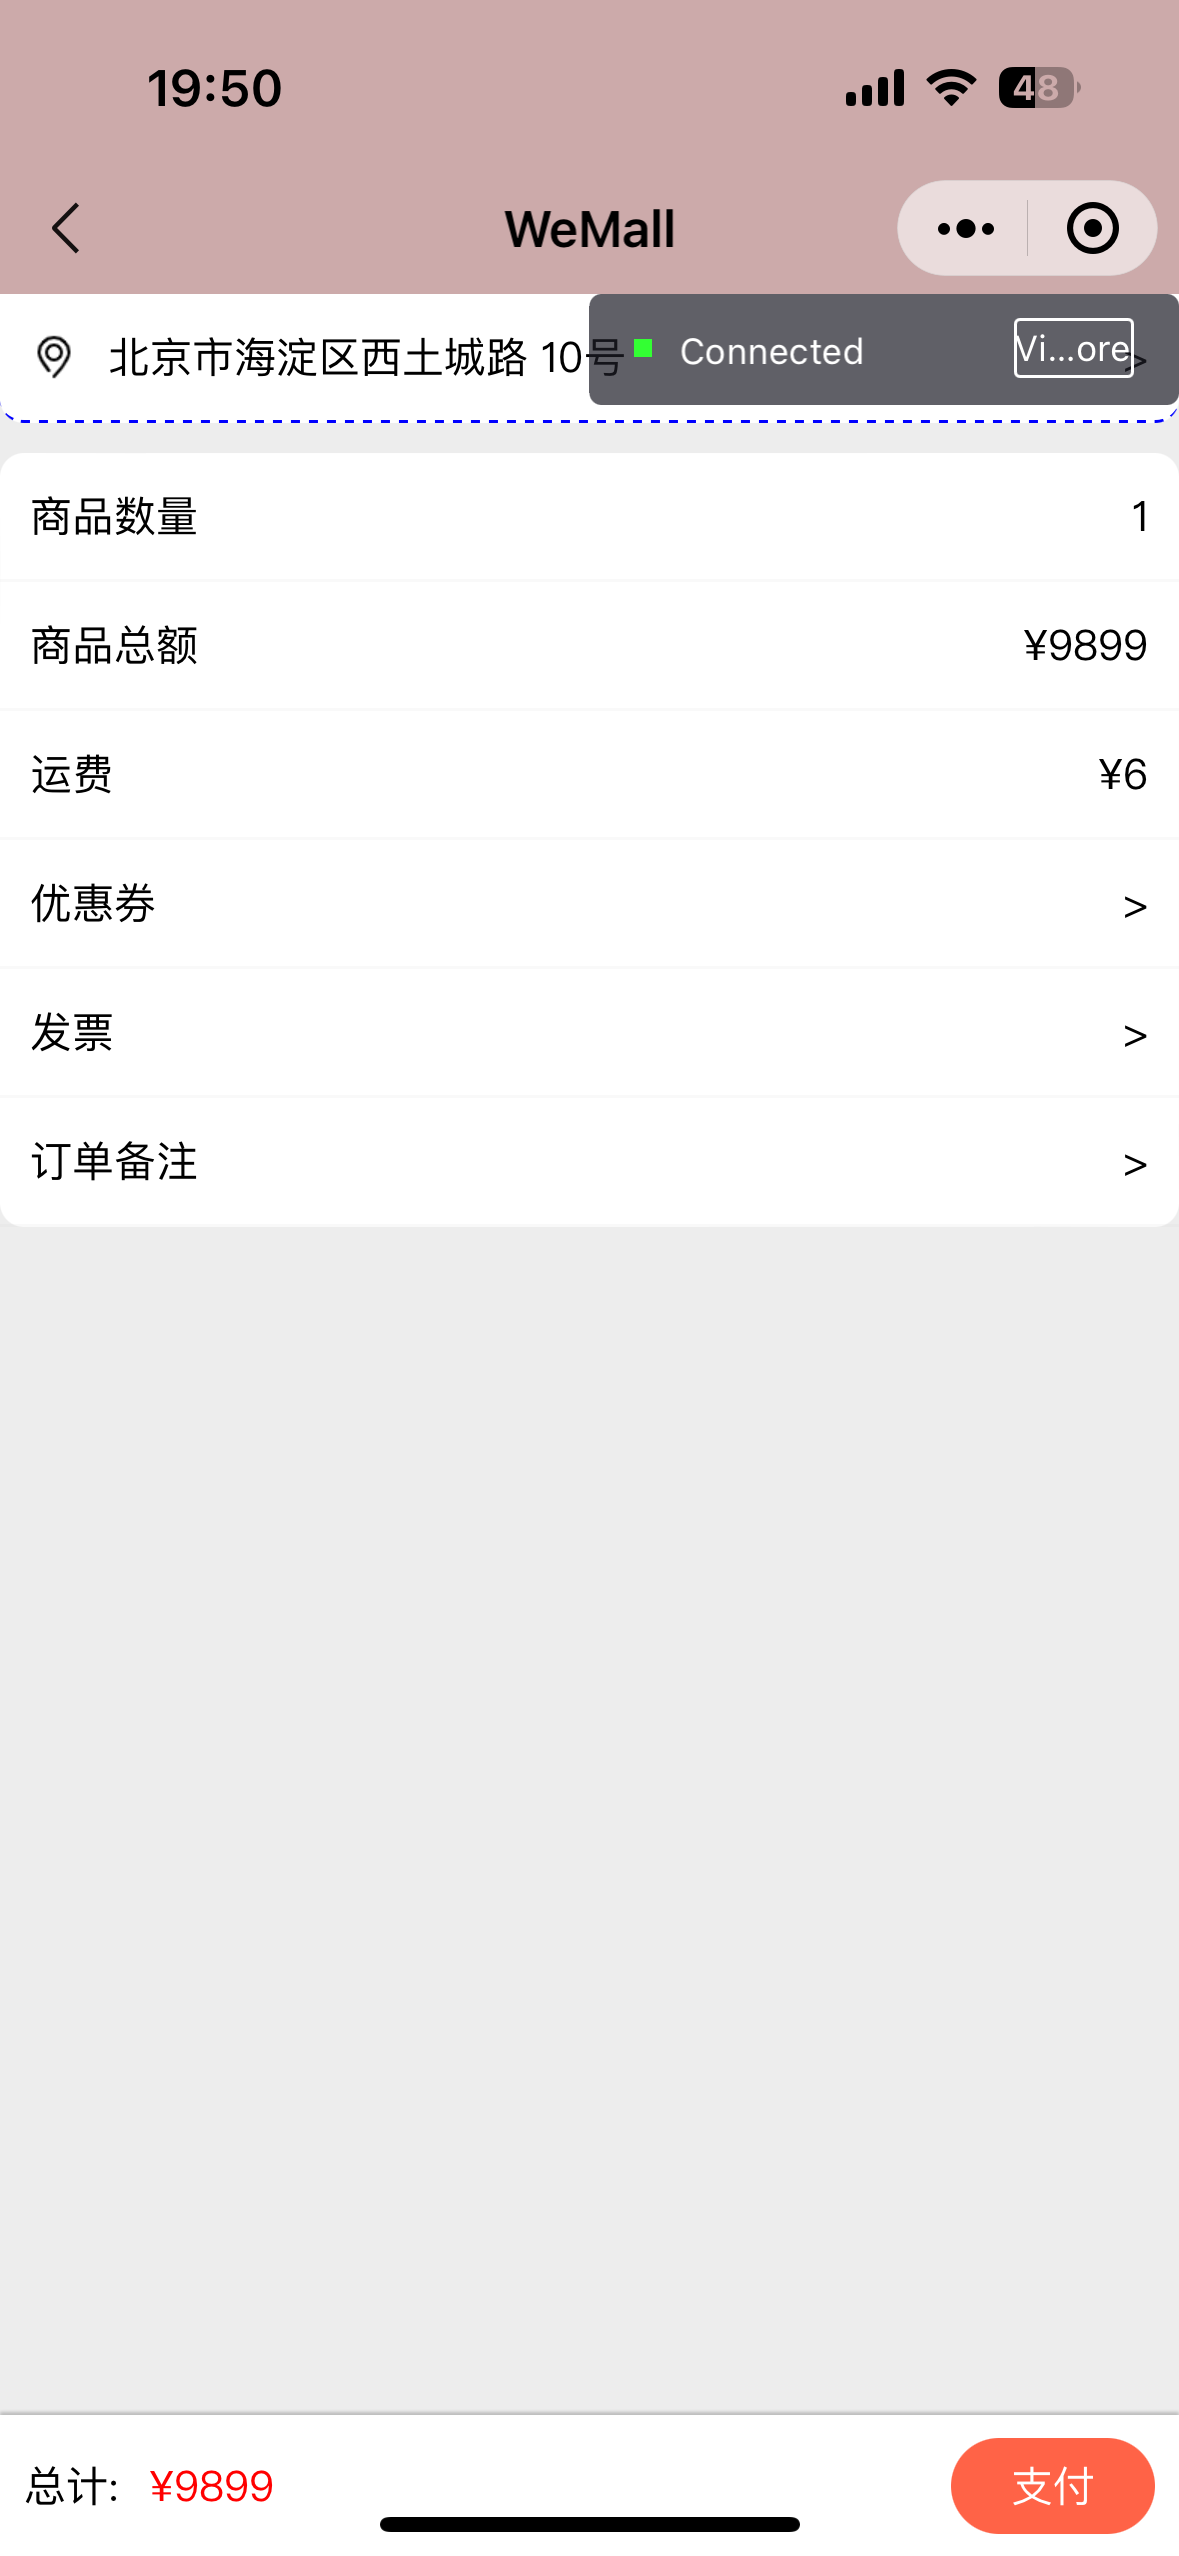
\includegraphics[width=0.4\textwidth]{2.jpg}
        }
    \end{figure}
    \begin{figure}[htbp]    % 常规操作\begin{figure}开头说明插入图片
        \centering            % 前面说过,图片放置在中间
        \subfloat[进行支付]   % 第一张子图的下标(注意:注释要写在[]中括号内)
        {
            \label{fig:subfig3}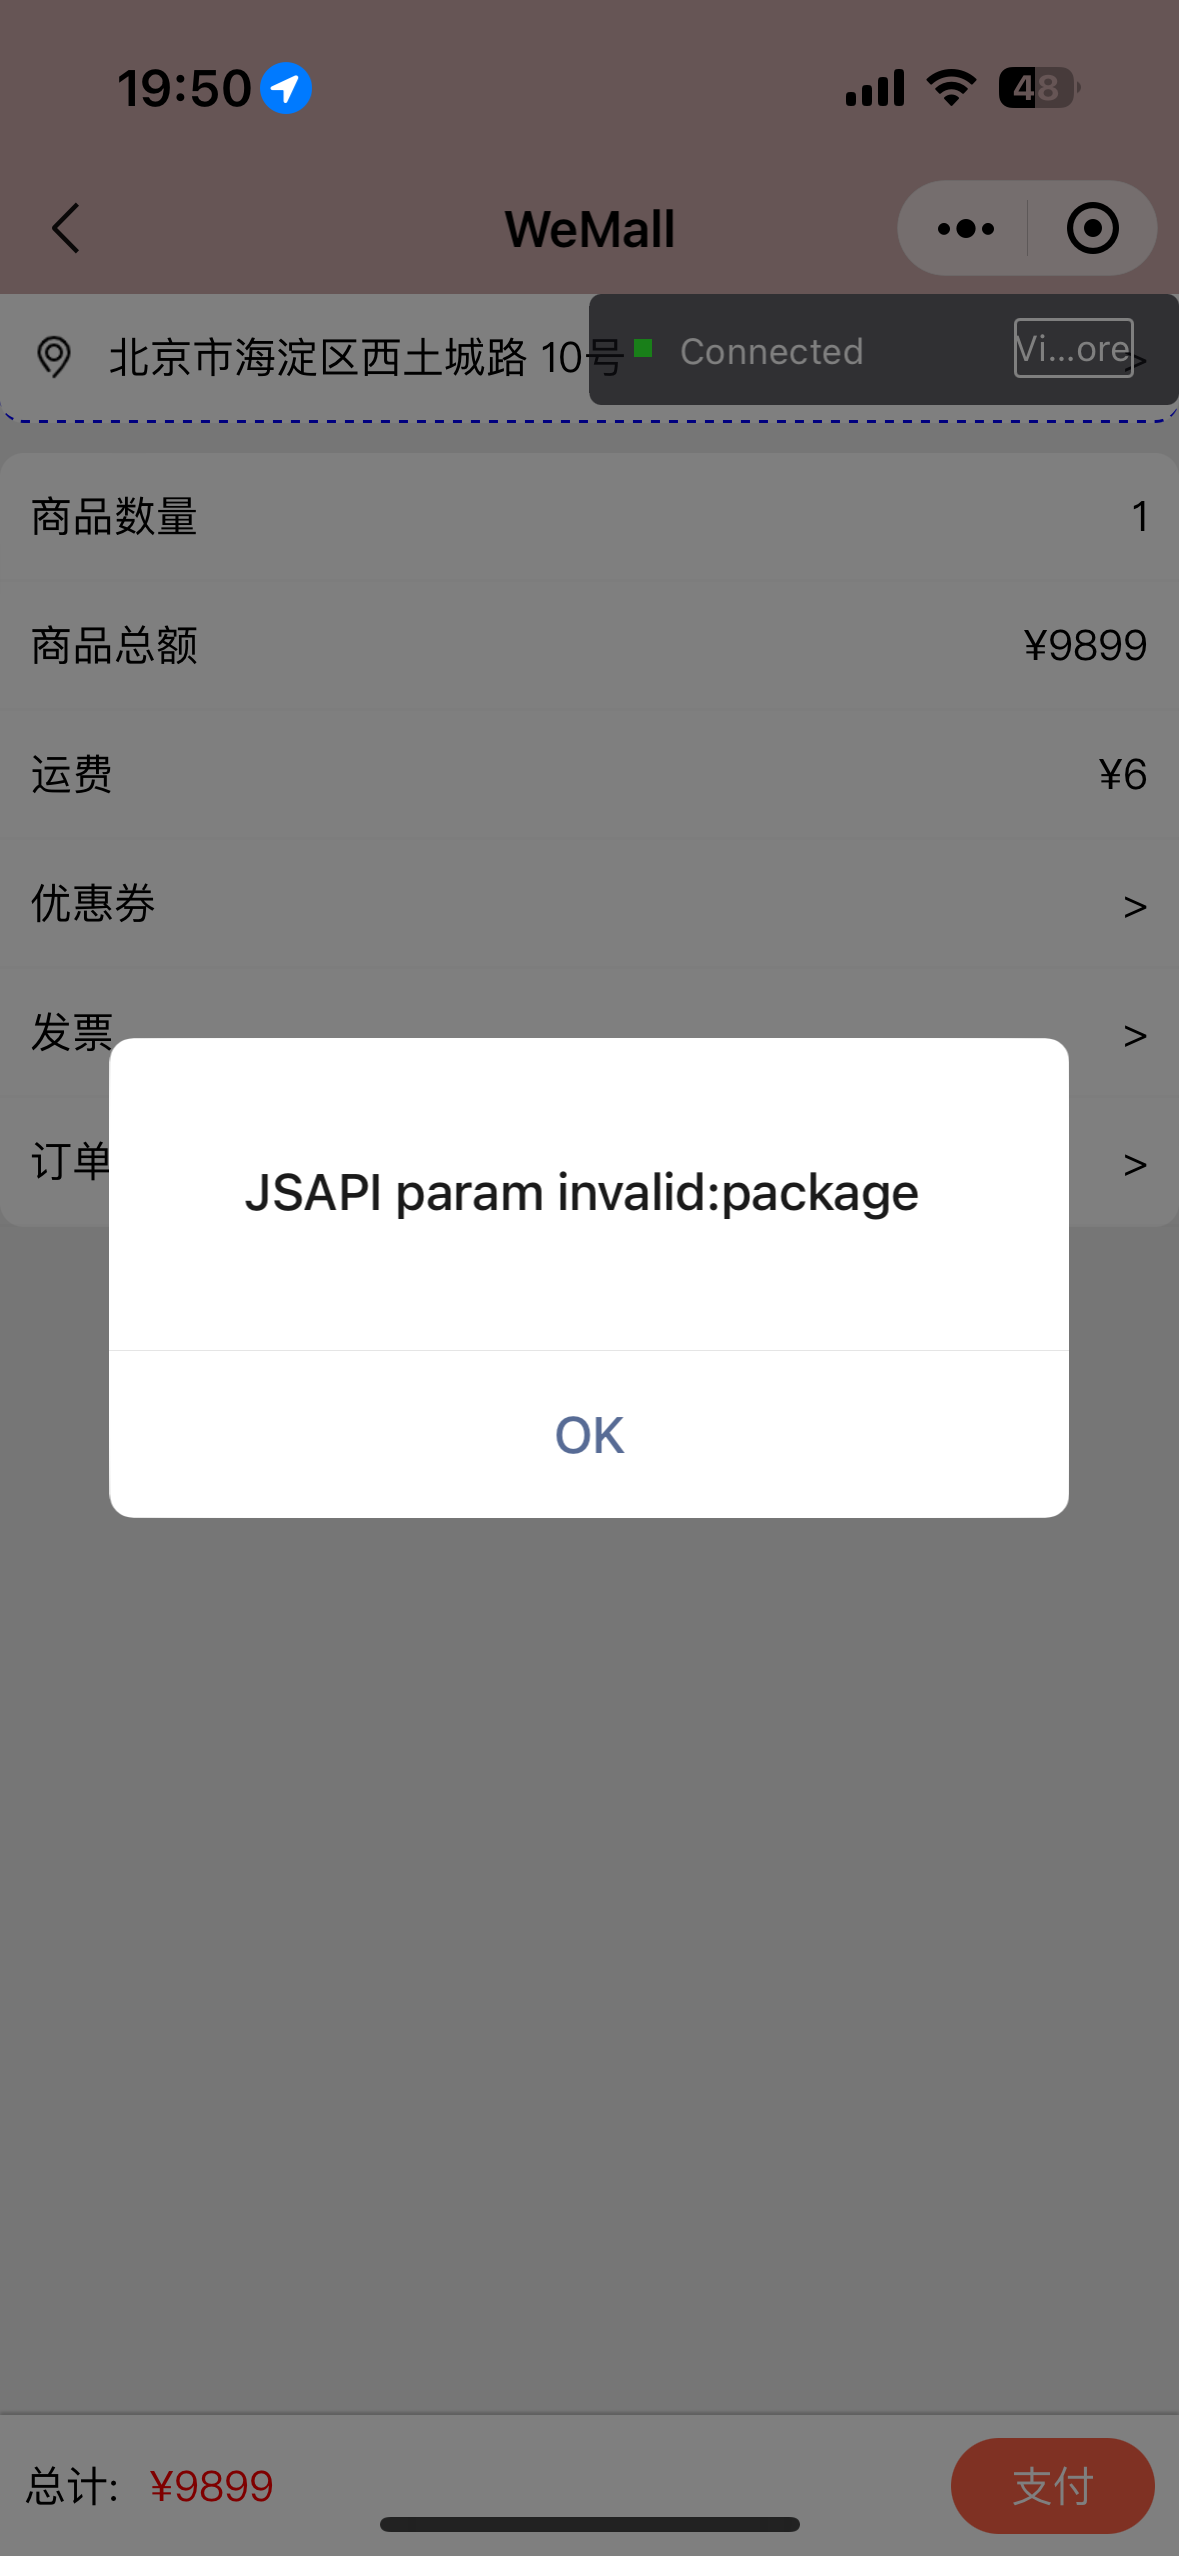
\includegraphics[width=0.4\textwidth]{3.jpg}
        }
        \subfloat[支付失败]
        {
            \label{fig:subfig4}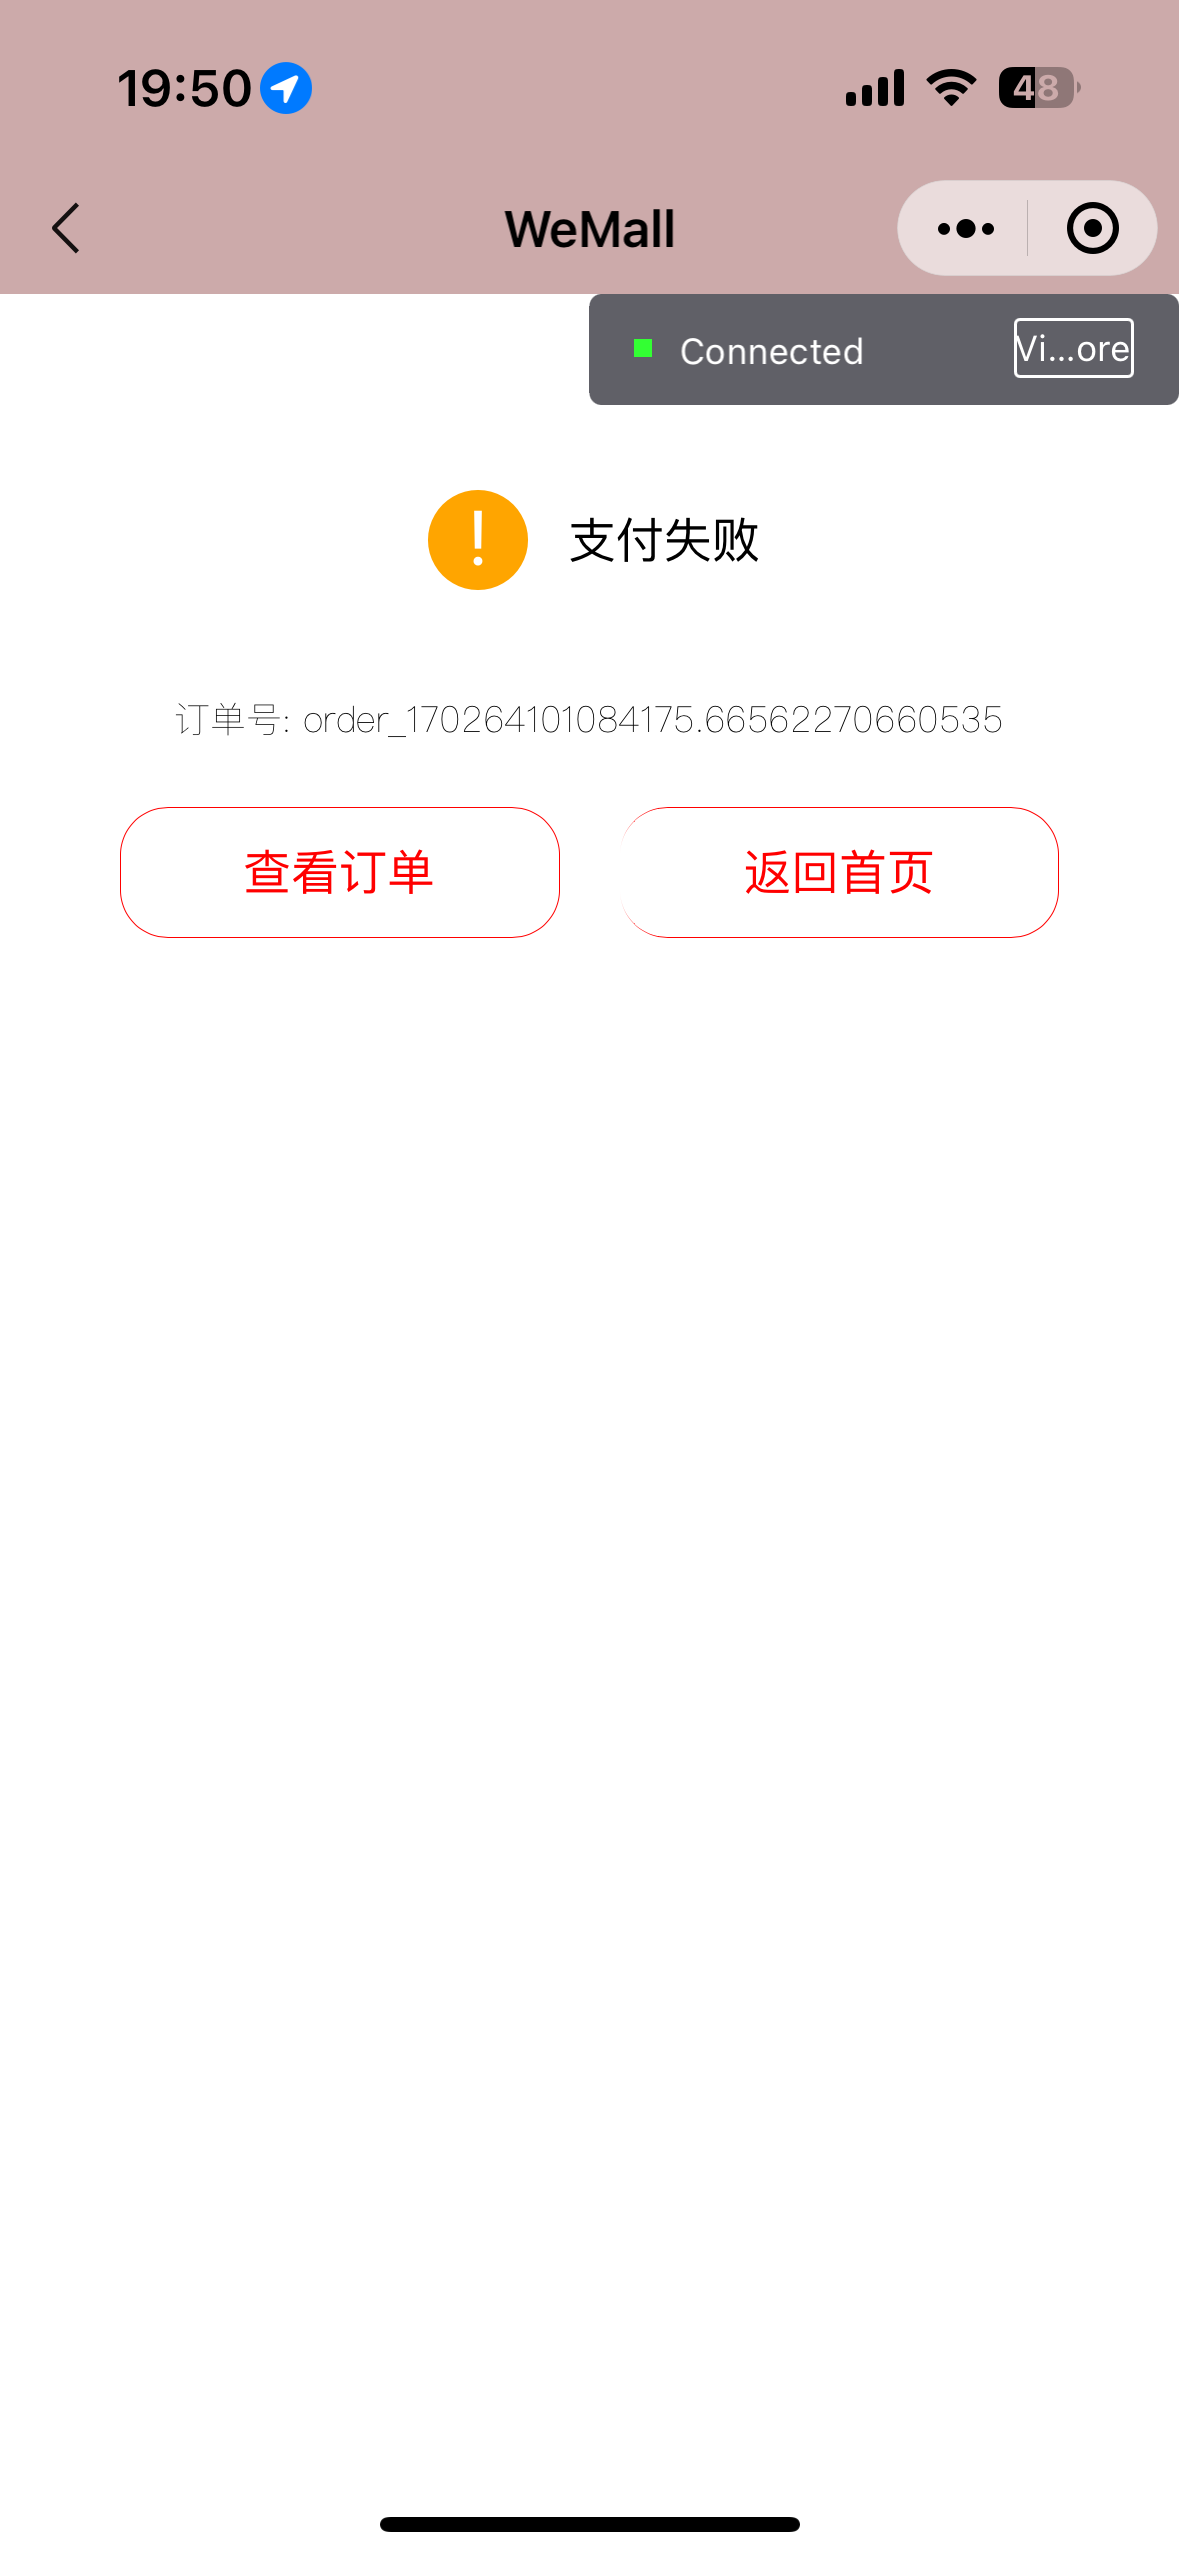
\includegraphics[width=0.4\textwidth]{4.jpg}
        }
    \end{figure}

